\section{ParSplice Keyspace Analysis}
\label{sec:parsplice-keyspace-analysis}
%IT HAS 8K keys!  How did we take these measurements

We instrumented ParSplice with performance counters and keyspace counters.  The
performance counters track ParSplice progress while keyspace counters track
which keys are being accessed by the ParSplice ranks. Because the keyspace
counters have high overhead we only turn them on for the keyspace analysis.
The cache hierarchy is unmodified but for the persistent database node, we
replace BerkeleyDB on NFS with LevelDB on Lustre. Original ParSplice
experiments showed that BerkeleyDB's syncs caused reads/writes to bottleneck on
the persistent database. We also use Riak's customized
LevelDB\footnote{https://github.com/basho/leveldb} version, which comes
instrumented with its own set of performance counters.

All experiments ran on Trinitite, a Cray XC40 with 32 Intel Haswell 2.3GHz
cores per node.  Each node has 128GB of RAM and our goal is to limit the size
of the cache to 3\% of RAM\footnote{Empirically, this is a threshold that we
find to work well for most applications}. Note that this is an addition to the
30GB that ParSplice uses to manage other ranks on the same node.  A single Cray
node produced trajectories that are \(5\times\) times longer than our 10 node
CloudLab clusters and \(25\times\) longer than UCSC's 10 node cluster. As
a result, it reaches different job phases faster and gives us a more
comprehensive view of the workload. The performance gains compared to the
commodity clusters have more to do with memory/PCI bandwidth than network.

\begin{figure}[t]
  \noindent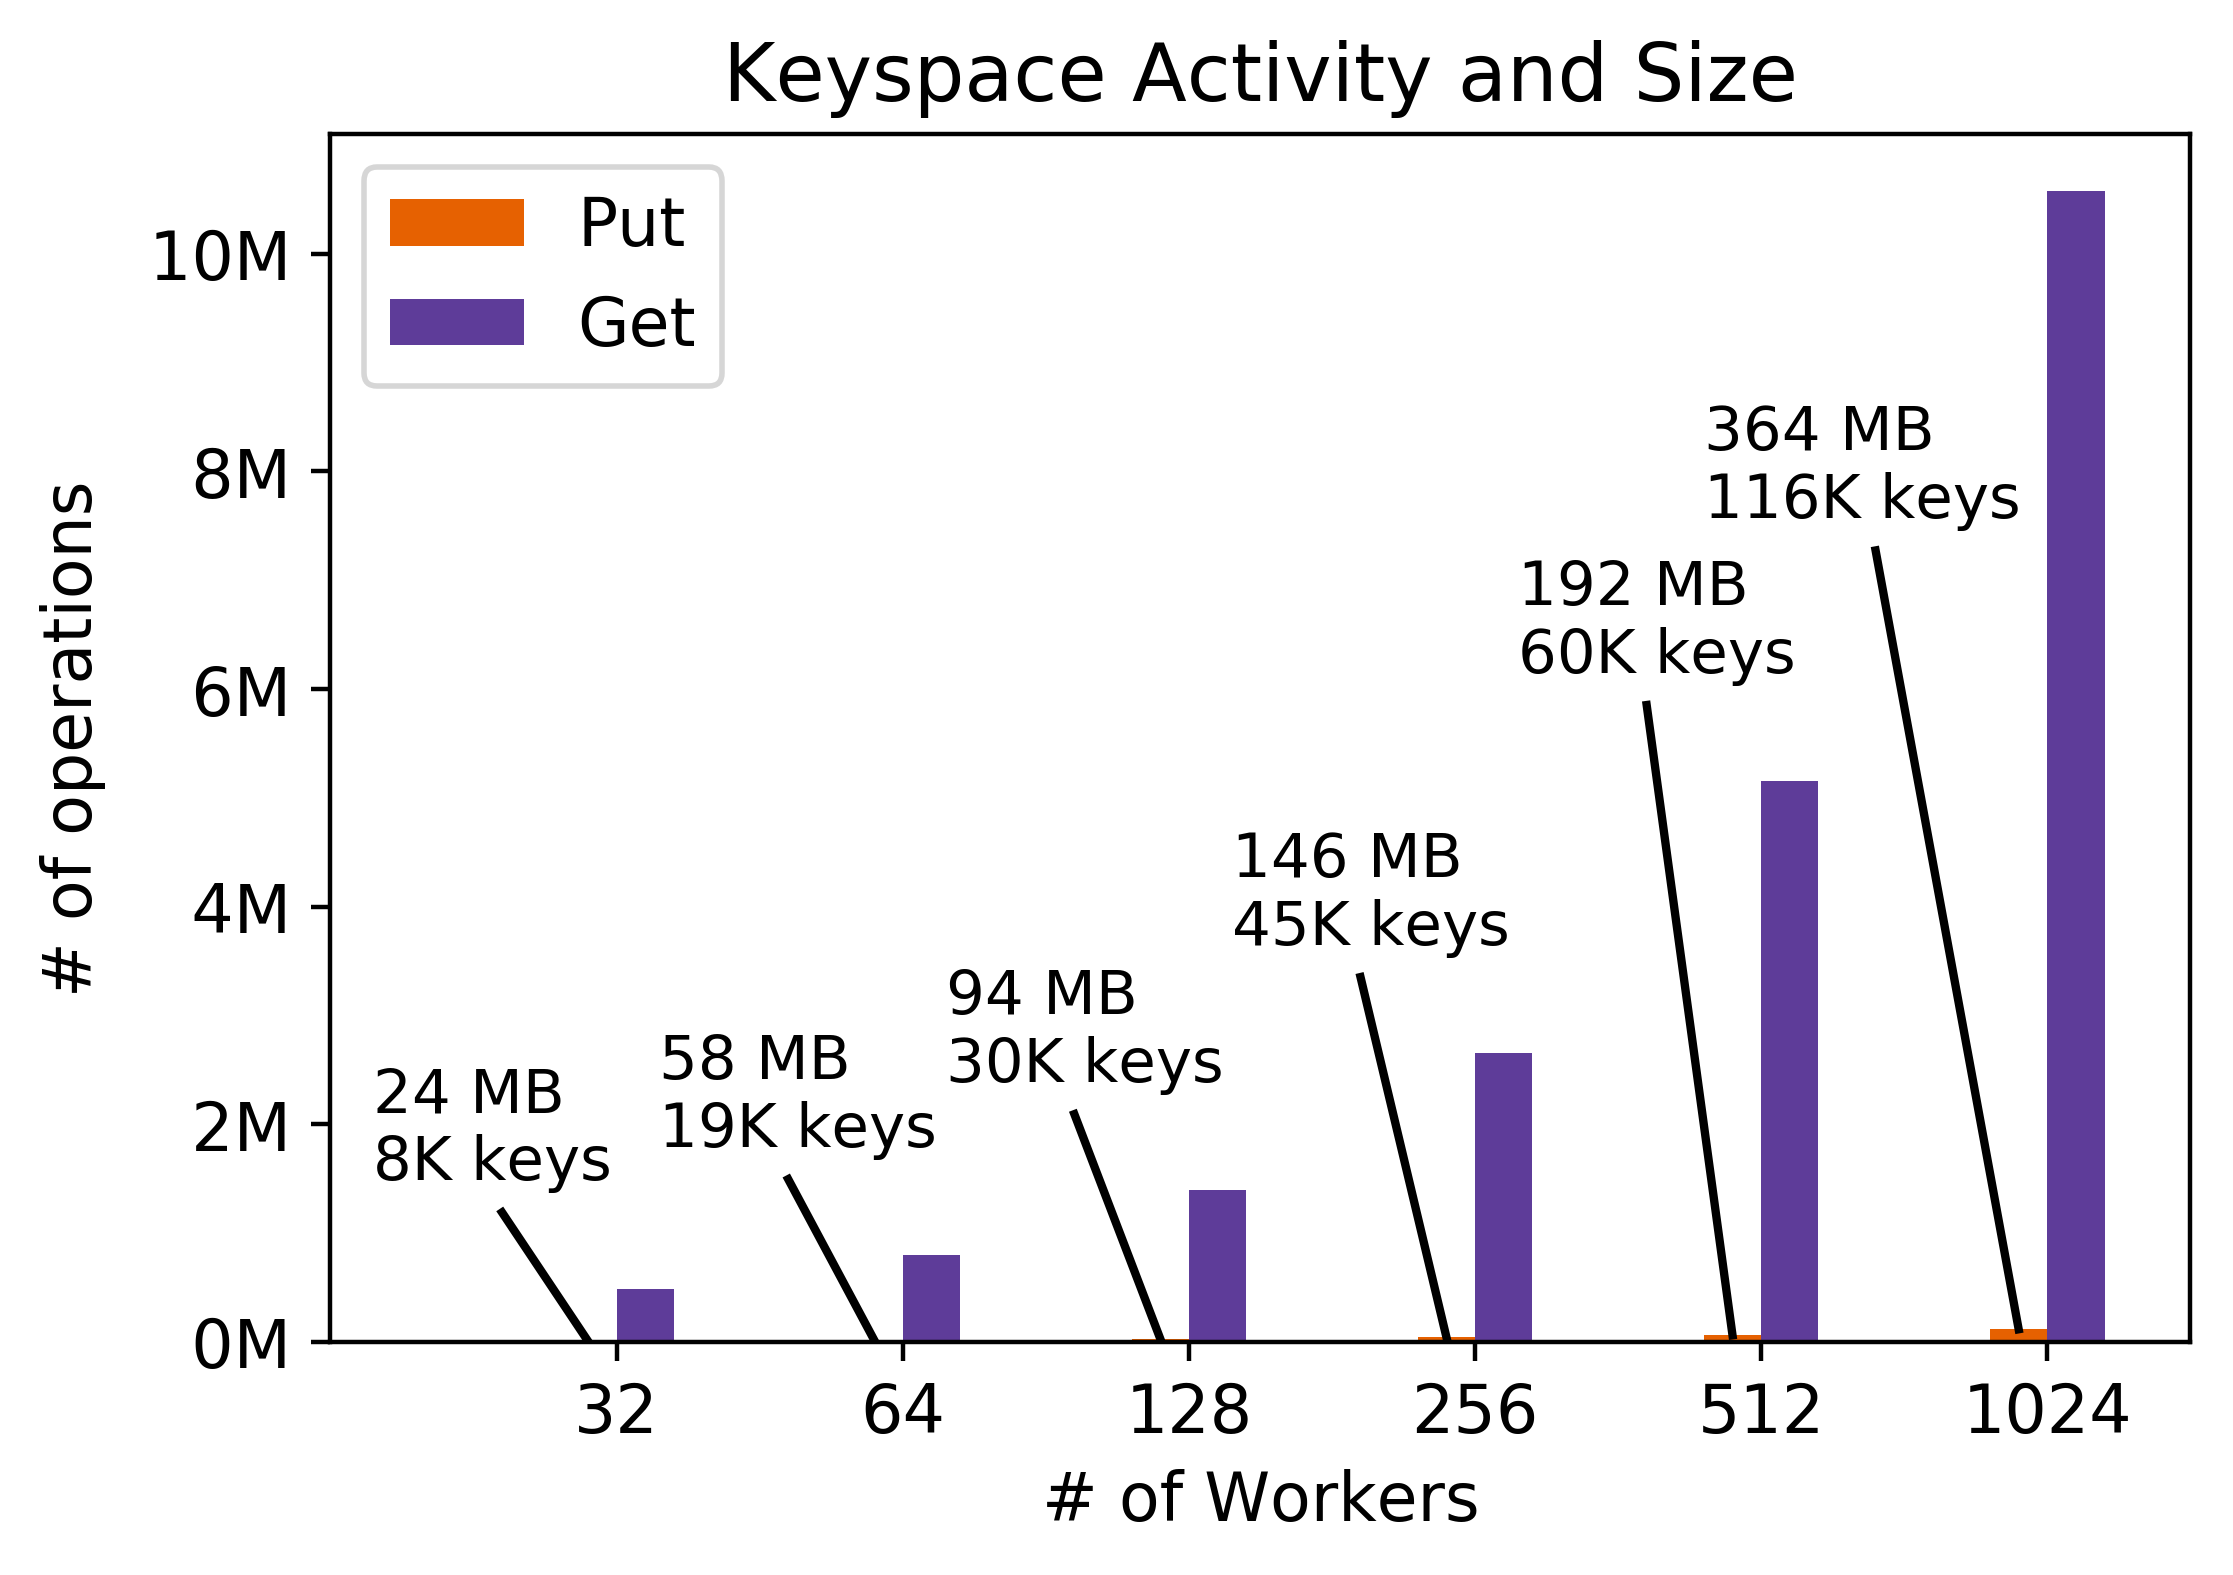
\includegraphics[width=0.5\textwidth]{figures/methodology-keyspace.png}\\
  \caption{The keyspace size is small but must satisfy many reads as workers
  calculate new segments. It is likely that we will need
  more than one node to manage segment coordinates when we scale the system or jobs up.
  \label{fig:methodology-keyspace}}
\end{figure}

\begin{figure}[t]
  \noindent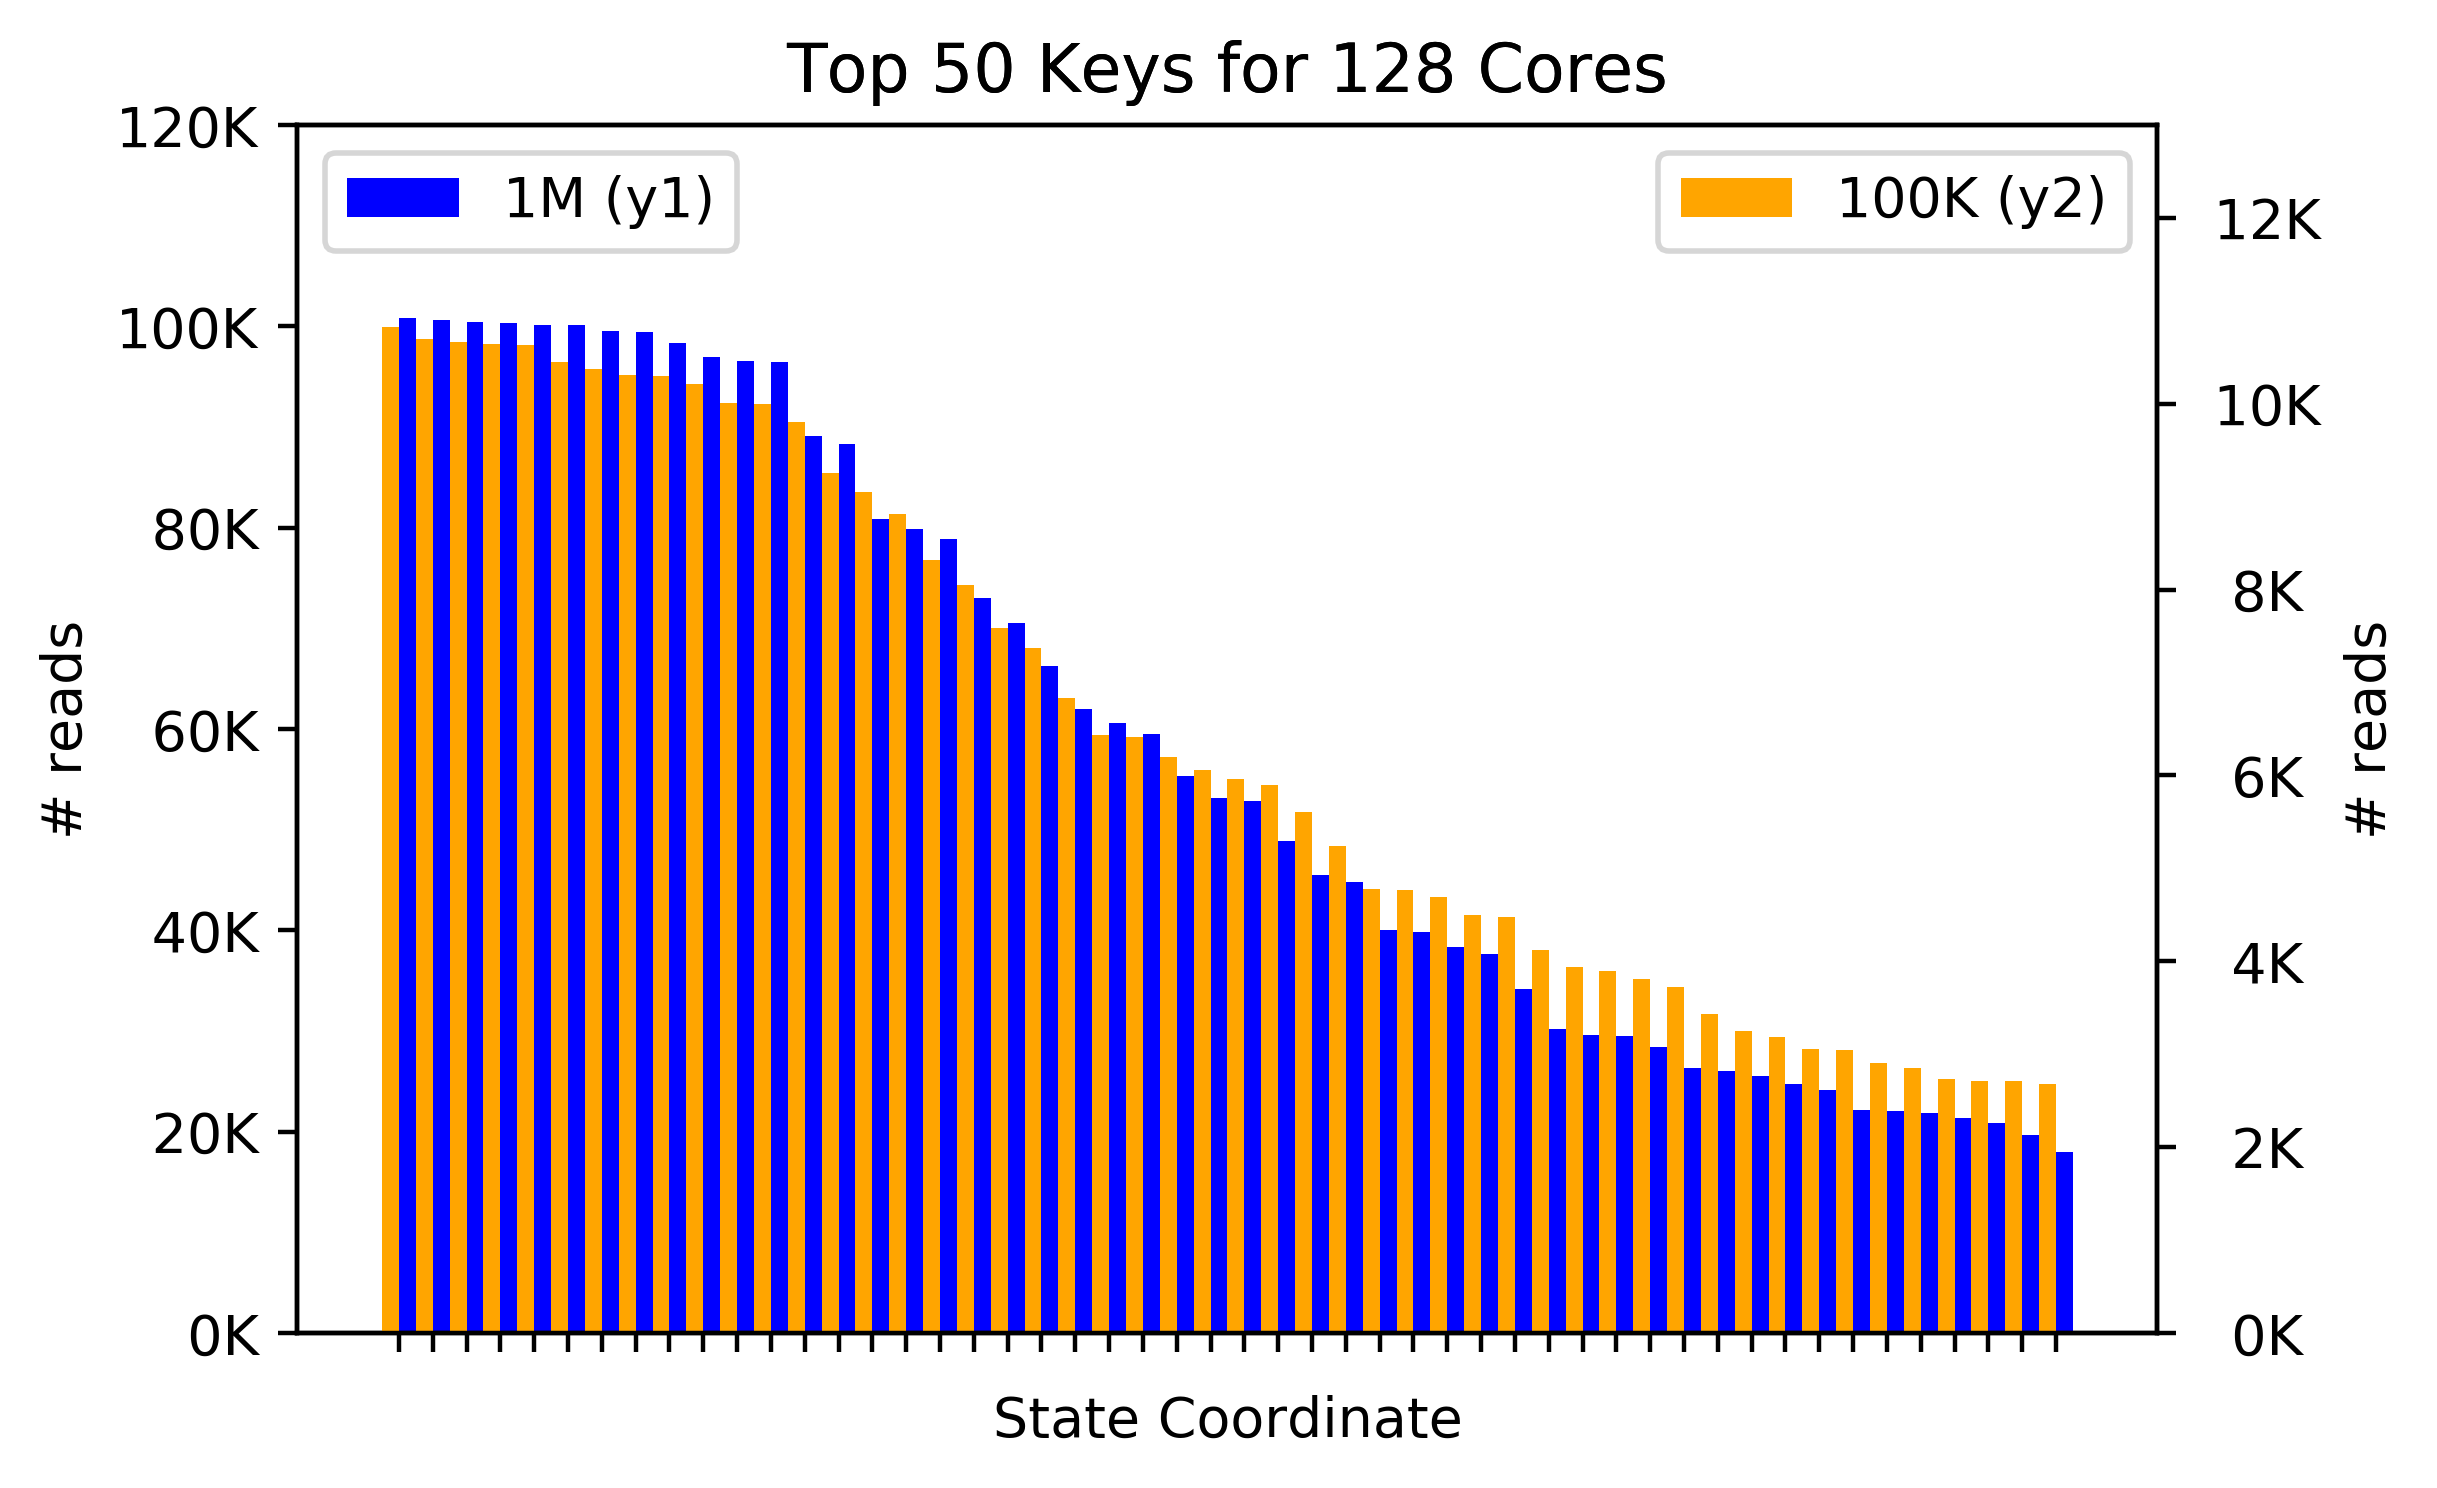
\includegraphics[width=0.5\textwidth]{figures/methodology-keys.png}\\
  \caption{The keyspace imbalance is due to workers generating deep
  trajectories and reading the same coordinates. Over time, the accesses get
  dispersed across different coordinates resulting in some keys being more
  popular than others.\label{fig:methodology-keys}}
\end{figure}

\subsubsection*{Scalability} Figure~\ref{fig:methodology-keyspace} shows the
keyspace size (black annotations) and request load (bars) after a one hour run
with a different number of workers (\(x\) axis). While the keyspace size and
capacity is relatively modest the memory usage scales linearly with the number
of workers. This is a problem if we want to scale to Trinitite's 6000 cores.
Furthermore, the size of the keyspace also increases linearly with the length
of the run.  Extrapolating these results puts an 8 hour run across all 100
Trinitite nodes at 20GB for the cache.  This memory utilization easily eclipses
the 3\% threshold we set earlier, even without factoring in the memory usage
from other workers.

\subsubsection*{An active but small keyspace} The bars in
Figure~\ref{fig:methodology-keyspace} show \(50-100\times\) as many reads
(\texttt{get()}) as writes (\texttt{put()}).  Worker tasks read the same key
for extended periods because the trajectory can remain stuck in so-called
superbasins composed of tightly connected sets of states. In this case, many
trajectory segments with the same coordinates are needed before the trajectory
moves on.  Writes only occur for the final state of segments generated by
worker tasks; their magnitude is smaller than reads because the caches ignore
redundant write requests. The number of read and write requests are highest at
the beginning of the run when worker tasks generate segments for the same
state, which is computationally cheap (this motivates
Section~\S\ref{sec:static-load-balancing}).

\subsubsection*{Entropy increases over time} The reads per second in
Figure~\ref{fig:motivation-regimes} show that the number of requests decreases
and the number of active keys increases over time. The resulting key access
imbalance for the two growth rates in Figure~\ref{fig:motivation-regimes} are
shown in Figure~\ref{fig:methodology-keys}, where reads are plotted for each
unique state, or key, along the \(x\) axis. Keys are more popular than others
(up to \(5\times\)) because worker tasks start generating states with different
coordinates later in the run (this motivates
Section~\S\ref{sec:the-need-for-dynamic-load-balancing-policies}).  The growth
rate, temperature, and number of workers have a predictable effect on the
structure of the keyspace.  Figure~\ref{fig:methodology-keys} shows that the
number of reads changes with different growth rates, but that the spatial
locality of key accesses is similar ({\it e.g.}, some keys are still
\(5\times\) more popular than others).  Figure~\ref{fig:motivation-regimes}
shows how entropy for different growth rates has temporal locality, as the
reads per second for \(\Delta_2\) looks like the reads per second for
\(\Delta_1\) stretched out along the time axis.  Trends also exist for
temperature and number of workers but are omitted here for space. This
structure means that we can learn the regimes and adapt the storage system
(this motivates Section~\S\ref{sec:ml-for-the-keyspace}).
